\documentclass[]{article}

\usepackage{amssymb}
\usepackage{amsthm}
\usepackage{amsmath}
\usepackage{pgfplots}
\usepackage{tikz}
\usepackage[margin=0.8in]{geometry}
\usepackage{scrextend}

\begin{document}
\begin{center}
	Simple table:\\
	\begin{tabular}{|c|c|c|c|c|}
		\hline
		a & b & c & d & e \\ \hline
$f$ & $g$ & $h$ & $i$ & $j$ \\ \hline

	\end{tabular}
\end{center}

\begin{center}
	Table with lookup:\\
	\begin{tabular}{|c|c|c|c|c|c|}
		\hline
		Mode/Letter & Letter 1 & Letter 1 & Letter 1 & Letter 1 & Letter 1 \\ \hline
No Math Mode & a & b & c & d & e \\ \hline
Math Mode & $f$ & $g$ & $h$ & $i$ & $j$ \\ \hline

	\end{tabular}
\end{center}

\begin{center}
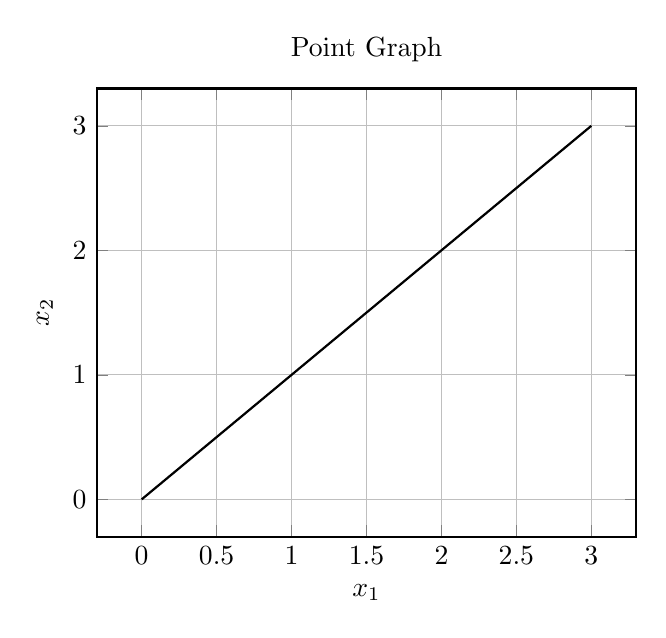
\begin{tikzpicture}
	\begin{axis}[xlabel = $x_1$, ylabel = $x_2$, title = Point Graph, grid=both, mark size = 3, thick]
	\addplot [black] coordinates {
(0.000000,0.000000)
(1.000000,1.000000)
(2.000000,2.000000)
(3.000000,3.000000)
};
\end{axis}
\end{tikzpicture}
\end{center}

\begin{center}
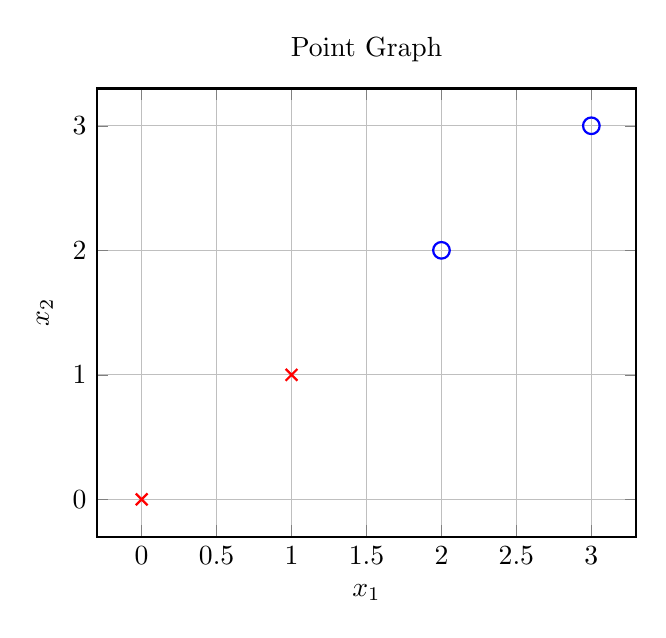
\begin{tikzpicture}
	\begin{axis}[xlabel = $x_1$, ylabel = $x_2$, title = Point Graph, grid=both, mark size = 3, thick]
	\addplot+[only marks, mark=o] coordinates{
(2.000000,2.000000)
(3.000000,3.000000)
};
\addplot+[only marks, mark=x] coordinates{
(0.000000,0.000000)
(1.000000,1.000000)
};

\end{axis}
\end{tikzpicture}
\end{center}

\end{document}